\section{Problem formulation}\label{sec:problem}

\subsection{Forward model of the traps}

The SLM has $N\times N$ pixels of pitch $p$ and is lit by a Gaussian beam of amplitude $A_j$ on pixel $j$, normalized so that $\sum_jA_j^2=N^2$. A hologram is a phase $\phi_j\in[0,2\pi)$ on each pixel, at position $(x_j,y_j)$ from the optical axis.
A lens of focal length $f$ at wavelength $\lambda$ forms the traps in its focal plane. For a trap $m$ at $(x_m,y_m)$ in that plane, with no axial offset and no vortex, the complex amplitude and the intensity, as a fraction of the power of the input beam, are
\begin{equation}
V_m(\phi)=\frac1{N^2}\sum_jA_j\,e^{\,i(\phi_j-\Delta_j^m)},\qquad \Delta_j^m=\frac{2\pi}{\lambda f}\,(x_jx_m+y_jy_m),\qquad I_m(\phi)=|V_m(\phi)|^2,\label{eq:forward}
\end{equation}
which is the point-trap form of Di Leonardo et al.~\cite{dileonardo2007}. The map $\phi\mapsto V$ is smooth; its derivative with respect to a pixel phase is $\partial V_m/\partial\phi_j=iA_je^{i(\phi_j-\Delta_j^m)}/N^2$, a fact the gradient of Section~\ref{sec:proposed-method} uses.
For traps on the bins of the zero-padded fast Fourier transform of the SLM field, the same amplitudes are entries of that transform, which is how the engine of the product evaluates the large benchmark cases; the experiments of this paper evaluate Eq.~\eqref{eq:forward} directly.
The array is a set of $M$ traps with positive weights $w_m$ that state the intended relative intensities; the task of the experiments has $M=100$ traps of equal weight.

\subsection{Residual aberrations}

The optical train between the SLM and the focal plane adds a wavefront error. Expanded in the Zernike modes $Z_k$ in Noll order~\cite{noll1976}, orthonormal over the disc inscribed in the SLM, it is $W(a)=\sum_ka_kZ_k$ with coefficients $a_k$ in waves, and the unit rms of
each mode means that the rms wavefront error is the root sum of squares of the coefficients. The aberration adds a phase offset to the displayed hologram, as in the total-phase sum of Nogrette et al.~\cite{nogrette2014}:
\begin{equation}
\psi_j(a)=2\pi\sum_{k\in\mathcal K}a_k\,Z_k(x_j,y_j),\qquad I_m(\phi,a)=\big|V_m(\phi+\psi(a))\big|^2,\label{eq:aberrated}
\end{equation}
where $\mathcal K$ is the set of modes that remain after a correction. A correction removes piston, the two tilts (which move the pattern), and the part of the wavefront that was measured; we take the residual in the eight modes of Noll indices 4 to 11 (defocus, two astigmatisms,
two comas, two trefoils and primary spherical), with independent Gaussian coefficients $a_k\sim\mathcal N(0,s^2)$. The prior is a stated parameter and not a measurement of an instrument: $s=\parAb$ waves per mode gives an rms wavefront of $s\sqrt{8}=\parAbRms$ waves and a Strehl ratio of about $0.88$ by the exponential approximation of the
Strehl ratio in terms of the phase variance~\cite{mahajan1983}. Its value is the choice of the product and not a figure sourced from a published instrument, because the residual distribution depends on the device. Figure~\ref{fig:modes} shows the eight modes on the SLM disc: the rotationally symmetric defocus and spherical modes, the two astigmatisms, the two comas and the two trefoils, each normalized to unit rms so that a coefficient of one wave is one wave rms of that mode.

\begin{figure}[t]
\centering
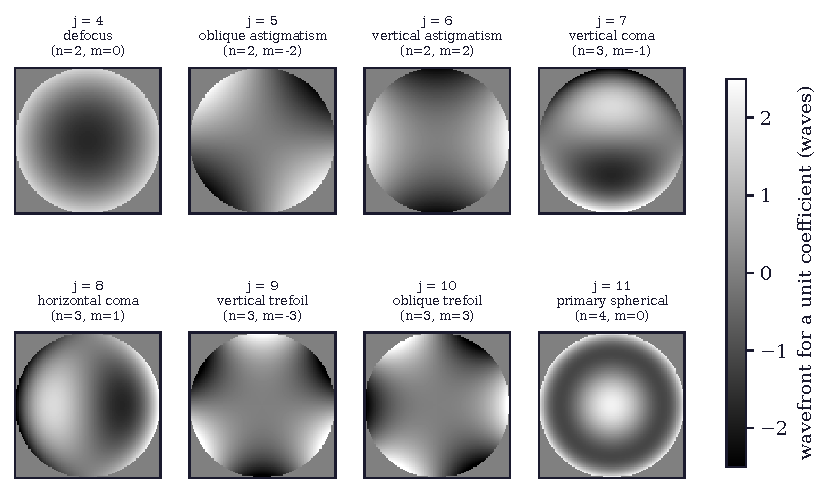
\includegraphics[width=0.9\textwidth]{fig-modes.pdf}
\caption{The eight aberration modes of the design (Noll 4 to 11) on the disc inscribed in the SLM, each for a unit coefficient of one wave, from the basis of the engine; the corners outside the disc are zero. Lighter and darker regions are phase advance and delay, in waves.}
\label{fig:modes}
\end{figure}

\subsection{Metrics and the quantity to be controlled}

Three quantities describe a hologram under a given aberration. The efficiency is the fraction of the input power in the traps, the spread is the relative standard deviation of the weighted intensities across the traps, and the cost compares the intensities with a target level:
\begin{equation}
e=\sum_mI_m,\qquad \sigma=100\,\frac{\operatorname{std}_m\!\big(I_m/w_m\big)}{\operatorname{mean}_m\!\big(I_m/w_m\big)},\qquad L(\phi,a)=\frac{\sum_m\big(I_m(\phi,a)-T_m\big)^2}{\sum_mT_m^2},\quad T_m=\ell\,e_0\,\frac{w_m}{\sum_nw_n},\label{eq:metrics}
\end{equation}
with $\sigma$ in percent, $e_0$ the efficiency of the starting hologram and $\ell$ the target level, a fraction of $e_0$. The spread $\sigma(\phi,a)$ is a random variable when $a$ is random, and what an experimenter fears is its upper tail: a draw of the residual aberration for which the array is uneven.
We therefore score a hologram by the 95th percentile $Q_{95}$ of $\sigma$ over an ensemble of draws of $a$, and by the mean efficiency over the same ensemble, and we compare two holograms by the ratio
\begin{equation}
\rho=\frac{Q_{95}\big[\sigma(\phi_{\mathrm{nom}},a)\big]}{Q_{95}\big[\sigma(\phi,a)\big]},\qquad \eta=\frac{\bar e(\phi)}{\bar e(\phi_{\mathrm{nom}})},\label{eq:ratios}
\end{equation}
where $\phi_{\mathrm{nom}}$ is the hologram of the published method that serves as baseline. A value $\rho>1$ means a lower tail of the spread, $\eta<1$ means a loss of efficiency, and the product tests the pair against $\rho\ge1.25$ and $\eta\ge0.9$ (Section~\ref{sec:design}).

\subsection{The design problem and its assumptions}

The design problem is to find the phase $\phi$ that minimizes the expected cost over the prior of the residual aberration,
\begin{equation}
\min_{\phi\in[0,2\pi)^{N\times N}}\ J(\phi)=\mathbb E_{a\sim\mathcal N(0,s^2I_8)}\,L\big(\phi,a\big),\label{eq:problem}
\end{equation}
and then to evaluate $\rho$ and $\eta$ on draws of $a$ that the optimizer did not use. The assumptions are listed because each bounds the result. (i) The scalar Fourier model of Eq.~\eqref{eq:forward} holds: the traps are on the ideal point-trap model, with no device model (no
pixel crosstalk, no phase quantization, no fill factor) in the forward map. (ii) The aberration is a phase offset on the SLM plane, as in the total-phase sum of the sources; the amplitude of the beam does not change. (iii) The coefficients are independent and Gaussian with one common scale. (iv) The ensemble that evaluates the hologram is drawn
from the same prior as the one that designs it, with a different seed and a different realization of the draws; robustness to other distributions is measured in Section~\ref{sec:results} and is not assumed. (v) The target level and the weights are known and fixed, and the traps are where they are meant to be.

\subsection{Notation}

Table~\ref{tab:notation} collects the symbols of the paper. Every symbol is defined where it first appears in the text, and the table fixes the unit of each one. Hologram phases and aberration phases are in radians, the Zernike coefficients in waves (one wave is $2\pi$ radians of phase), distances in the focal plane in focal bins, that is in units of $\lambda f/(\mathrm{pad}\,N\,p)$, the spacing of the samples of the zero-padded Fourier transform of the SLM field, and intensities as fractions of the power of the input beam, so that the efficiency is a fraction and the spreads are percentages. Indices $j$ run over the SLM pixels, $m$ over the traps and $k$ over the designed modes. The symbols $L$ and $J$ always refer to the cost of Eq.~\eqref{eq:metrics} and its expectation, and $\sigma$ is always the spread of the trap intensities of one realization and not a standard deviation of a prior.

\begin{table}[t]
\centering\small
\caption{Notation of the paper: each symbol with its meaning and its unit; the defaults of the product are the values of the design in Table~\ref{tab:params}.}
\label{tab:notation}
\begin{tabular}{@{}p{2.2cm} p{9.4cm} p{2.6cm}@{}}
\toprule
Symbol & Meaning & Unit\\
\midrule
$N$, $p$ & SLM side in pixels, pixel pitch & 1, \si{\micro\metre}\\
$\phi_j$, $A_j$ & hologram phase and input amplitude of pixel $j$ ($\sum_jA_j^2=N^2$) & rad, 1\\
$\lambda$, $f$ & wavelength, focal length of the lens & \si{\nano\metre}, \si{\milli\metre}\\
$M$, $w_m$ & number of traps, weight of trap $m$ & 1, 1\\
$V_m$, $I_m$ & amplitude and intensity of trap $m$ as a fraction of the input power & 1\\
$Z_k$, $a_k$ & Zernike mode of Noll index $k$ (unit rms over the disc), its coefficient & 1, waves\\
$\psi_j(a)$ & aberration phase on pixel $j$ & rad\\
$s$ & standard deviation of each coefficient in the prior (design amplitude) & waves\\
$\mathcal K$, $K$ & set of designed modes (Noll 4 to 11), their number & 1\\
$e$, $e_0$, $\ell$ & efficiency, efficiency of the start, target level fraction & 1\\
$T_m$ & target intensity of trap $m$, Eq.~\eqref{eq:metrics} & 1\\
$L$, $J$ & cost at one aberration, expected cost & 1\\
$\sigma$, $Q_{95}$ & relative standard deviation of the weighted intensities, its 95th percentile over draws & percent\\
$\rho$, $\eta$ & ratio of the 95th percentiles, ratio of the mean efficiencies, Eq.~\eqref{eq:ratios} & 1\\
$G_{mk}$ & derivative of $I_m$ in the coefficient $a_k$ at the nominal system & 1 per wave\\
$\kappa$ & relative curvature of a trap intensity under displacement & per bin squared\\
\bottomrule
\end{tabular}
\end{table}
